
\documentclass[12pt, a4paper]{report}
\usepackage{graphicx}
\usepackage{amsmath}
\usepackage{float}


\title{\textbf{EE2703 : Applied Programming Lab \\ Final Exam 2019}} % Title

\author{Name of the students \\ Roll number} % Author name

\date{\today} % Date for the report

\begin{document}		
		
\maketitle % Insert the title, author and date
\section*{Q1}
 Input short summary of the question here which includes required  \textbf{formulas and facts and properties.} 
 
 \begin{equation}\label{eq:1}
 V_{n1}-V_{n2}=I_{n1,n2} R_{n1,n2}
 \end{equation}
 Multiple equations:
 \begin{align}
    f(x) &= x^{2-\alpha}\\
    g(x) &= \frac{1}{x}\\
    F(x) &= \int_{0}^{x} f(u)\,du\\
    f'(x) &= \frac{d}{dx}f(x)\\
    A    &= \begin{bmatrix}
            a_{1 1} & a_{1 0} \\
            a_{0 1} & a_{0 0}
           \end{bmatrix}\\
    \frac{\partial Q}{\partial t} &= \frac{\partial s}{\partial t}
 \end{align}
 To insert equation without numbering.
 \begin{equation*}
 V_{n1}-V_{n2}=L_{n1,n2} \frac{dI_{n1,n2}}{dt}
 \end{equation*}
 
 Here are some inline math: $ \alpha = \frac{\beta + \Phi (\phi) }{\Theta ( \theta )} $
 
 
 
 
 
 
\subsection*{Codes}
 To insert inline command you can use \texttt{print("Hello World")} \\
To type block of code manually use the following block
\begin{verbatim}	
x = fun1(x1, x2, x3)
z = fun2(z1, z2, z3)
print('x = %d and z = %d' % (x,z))
\end{verbatim}


\subsection*{Results}
Include all the plots asked in the question here.
 \begin{figure}[H]
	\centering
	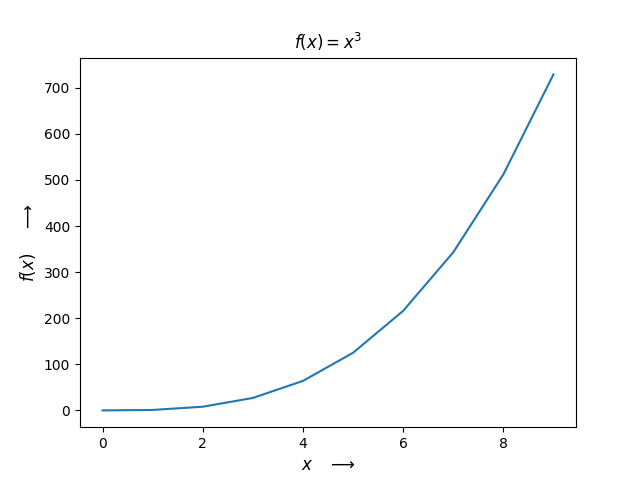
\includegraphics[scale=0.8]{Figure_1.png}  % Mention the image name within the curly braces. Image should be in the same folder as the tex file. 
	\caption{Sample image}
	\label{fig:sample}
\end{figure} 


\subsection*{Conclusions}
Figure~\ref{fig:sample} is the sample image  \\
Equation ~\ref{eq:1} is the sample equation 
   \begin{itemize}
  	\item One
  	\item Two
  \end{itemize}
  If you want to number them:
  \begin{enumerate}
      \item One 
      \item Two
  \end{enumerate}
% Repeat the above sections for the rest of the question. 

\end{document}



 